\documentclass[letterpaper]{article}

\usepackage[utf8]{inputenc}
\usepackage{amsmath}
\usepackage{listings}
\usepackage{hyperref}
% https://tex.stackexchange.com/questions/180571/making-clickable-links-to-sections-with-hyperref
\usepackage{graphicx}
\usepackage{comment}

\graphicspath{ {./images/} }

\title{A DSL for writing safer string manipulation functions in C}
\author{Michael Flanders}
\date{December 16, 2020}

%You can skip explaining the state of the art (i.e., how the problem is solved today).
%Instead, make sure to include a description of your language. Ideally,
%  you present a language tutorial using your previously selected examples. 
%When explaining your design, refer back to the architecture of DSL
%  implementations, similarly to how we asked you about the FFTW architecture
%  in the reading homework. 
%Please make your design description point to the relevant lines of your implementation.
%  Ideally, your doc will include links to the range of code in your github repo. 
%Please share the repo with the user rbodik. 
%Include the answers to the questions from the last slide.
%Please add the answer to the question "What knowledge or skill would have helped you
%  be more successful with the project."  The answers will help us in further upgrading
%  the course. 

\begin{document}
\maketitle

% Overview of project
% Overview of the sections

For this project, I built a DSL that prevents the common string and
integer related vulnerabilities and undefined behaviors in C programs.
The DSL is a small, restricted subset of C with some additional constructs
like $String$ types, iterators, range and subrange constraints, and bounded,
fold-style loops. By raising the abstraction level of strings and loops
and using the range constraints in typechecking and static analysis,
most of the common string vulnerabilities can be eliminated.

This report provides an \hyperref[sec:domain]{analysis of the problem domain (\S1)},
\hyperref[sec:language]{a description of the DSL (\S2)},
\hyperref[sec:design]{a breakdown of the design and design decisions made (\S3)},
and \hyperref[sec:discussion]{a discussion of the project (\S4)}.

\section{Domain analysis}
\label{sec:domain}

I built the DSL as a development aid for new or moderately experienced
C developers. These developers would be writing some C application
that needs to handle user input, and that user input is often a string.
The input validation, sanitization, and processing functions would be
written in the DSL, compiled to a header file, and then imported to
the project to help provide a stronger outer shell.

These security guarantees do have a cost since the performance of the
generated C code cannot compare to the performance that an experienced
C developer might be able to achieve. However, I would argue that even
using the DSL only on validation, sanitization, and pre-processing code would
provide a lot of security benefits while only having a slight performance
impact (since most of the program logic is probably not contained in these
routines).

\subsection{A motivating example}

There are many codebases that could benefit from having their input processing
code rewritten in the DSL, but here I provide only one such example where the
DSL beats static analyzers, symbolic execution, and fuzzers. I do not
provide code here since I think distributing decompiled, closed-source code
is not very legal, but the example is from a \href{https://www.zerodayinitiative.com/advisories/ZDI-19-866/}
{vulnerability I found in Netgear routers last year.}

Figure \ref{fig:minihttpd} shows a function from the mini\_httpd
HTTP server that decodes HTML-Url encoded strings. This
same code is used in thttpd which powers sites such as
images.paypal.com, garfield.com, drudgereport.com, and
the official website of the Sovereign Principality of Sealand.

Another notable user of mini\_httpd is Netgear. Earlier
models of Netgear routers (pre-2018), use a modified version of mini\_httpd
with modifications to the decoding and sanitization functions such as
the one shown in figure \ref{fig:minihttpd}. These modifications make connecting
to the router from the Netgear phone app simpler, but also introduce a
severe vulnerability that allows networks guests to execute arbitrary code
on the router as an administrator.


\begin{figure}
\centering
\begin{lstlisting}
  static void
  strdecode( char* to, char* from )
  {
    for ( ; *from != '\0'; ++to, ++from )
    {
      if ( from[0] == '%' && isxdigit( from[1] ) && isxdigit( from[2] ) )
      {
	*to = hexit( from[1] ) * 16 + hexit( from[2] );
	from += 2;
      }
      else
      *to = *from;
    }
    *to = '\0';
  }
\end{lstlisting}
\caption{Code snippet from mini\_httpd}
\label{fig:minihttpd}
\end{figure}

This is a case where the DSL would shine; static analyzers, symbolic
execution, and fuzzing would all miss the vulnerability. The vulnerability
is caused by an incorrect implementation of a check for contained substrings
and bad pointer arithmetic. However, there is no undefined behaviour or
out-of-bounds accesses, so static analyzers and tools like KLEE or CBMC
will not warn. The strings needed to trigger the vulnerability are also
very complex; the vulnerability requires providing valid URL's that the
server transforms into an exploit/payload during sanitization and validation.
By providing a very carefully crafted URL, an attacker can trick the server
into inserting a null-byte within a string buffer (this turns one string into
two and is called a poison null-byte vulnerability), performing validity checks on the
second string, and then using the first string. Complex dependencies on
network connections and the filesystem further complicate the situation for fuzzers.

Writing the validation and decoding functions in the DSL would have avoided
this vulnerability. Even though there is no guarantee on functional correctness
of programs written in the DSL, the high-level string functions remove the
need to worry about null bytes and terminators, so this vulnerability could not
even have been written. In other words, the \textit{pre-provided} string functions in the DSL
should always compile to safe and functionally correct C code which is enough
in this case.

\section{Language description}
\label{sec:language}

% Overview
% Paradigm, immutability, boundedness
% Language constructs, operators
% Ranges, subranges
% For loops

\subsection{Overview}

The language is a small subset of C with
additional constructs: range constraints on types, $String$ types instead
of char*, iterator types, and bounded, for-style for-loops. Additional changes
to the usual C semantics include making all variables immutable, assigning
default range constraints to non-constrained values, preventing recursion,
and removing  other confusing features of C such as assignments in conditional
checks, pointers, pointer arithmetic, and casting between non-numeric types.

I believe that raising string manipulation from char* operators to String
operations will remove most of the common string vulnerabilities. However,
there could still be problems when mixing integers and strings. For example,
a common way that buffer overflows occur is performing arithmetic on string
lengths and using the results to allocate new memory or bound string operations
like $strncmp$. Since many C developers default to using $int$ as their default
numeric type, signed values often make their way into the C std string functions
which operate on unsigned types. The castings that occur can result in allocating
too small buffers or copying too much data which can both cause serious vulnerabilities.

Since the generated C code will use some of these C std string functions, the DSL
needs to guarantee that no problematic integer behavior will happen. To check for
this behavior, I decided to use abstract interpretation using an interval domain.
Using the results from the analysis, I can check that, for example, when casting
from a signed type to an unsigned type, the signed value could not have been negative.
The range and subrange constraints help the abstract interpretation by reducing false
positives, simplifying some safety checks, and also add more meaning to the code.

The iterator and for-style for-loops are important because they prevent pointer
arithmetic and bound issues when iterating over arrays of strings and numbers.
As an example, the string split function returns an array of strings. If the DSL
left iterating over this array of strings to the usual C-style for-loops, the
code could still be vulnerable to out-of-bounds accesses and overflows. 

The other language features like immutability, lack of recursion, and lack of
explicit casts are just to futher simplify analyses and to make the developer's
life a bit easier.

\subsection{Syntax and semantics}

\subsubsection{Expressions}

The DSL provides the following string functions: ston (string-to-number), split,
equals, concat, append, and length. The equivalent ntos (number-to-string) is
provided for int types as well as the operators: $+$, $-$, $*$, $/$, $<$, $>$, $<=$,
$>=$, $!$, $\&\&$, and $||$. The DSL also provides the following operations on
iterator types: concat, first, and length.

I came up with these functions by rewriting string.h and writing my easy, medium,
and hard example programs using the DSL. I ended up getting rid of lots of other
string functions since they could just be built from these string functions as
syntactic sugar.

\subsubsection{Statements}

There are four statements in the DSL: for, if, return, and assignments. If, return
and assignments have their usual semantics, but the for loops are different. An example
for loop is shown in Figure \ref{fig:forloopsyntax}.

The values in the for-header
have a left hand side (LHS) and a right hand side (RHS) separated by a pipe. The LHS
must have 1 or 2 expressions of the form $varName : expr$ delimited by a comma. I
decided to allow the second iterator since I could not think of another way to compare
two strings or iterators in the DSL. If 2 iterators are specified in the LHS, then the
loop iterates until the shorter one is exhausted. The RHS requires the declaration of an
accumulator value, and this is a normal declaration except that it doesn't have to be
initialized or assigned a value. For example, in Figure \ref{fig:forloopsyntax},
\textit{int acc = 0} could also be written as \textit{int acc}, and values would get default values
of 0, empty string, or empty iterator.

The body of the for loop consists of 0 or more statements with one terminating
expression used to update the accumulator.

\begin{figure}[h]
\centering
\begin{lstlisting}
    for ( c1 : str1, c2 : str2 | int acc = 0 ) {
      ...optional statements...
      ...required terminating expression that updates acc...
    }
\end{lstlisting}
\caption{Example of for-loop syntax}
\label{fig:forloopsyntax}
\end{figure}

\subsubsection{Functions}

Declaring a function is done in the DSL similarly to how it is done in C.
The only addition are range constraints on the return value and arguments
as shown in Figure \ref{fig:functionsyntax}. In Figure \ref{fig:functionsyntax},
the return value must be of type \textit{uint8\_t} and must be contained in
the inclusive interval $[0, 255]$. The argument \textit{numbers} is an iterator
over \textit{int32\_t} types. The iterator can hold at most 50000 numbers (inclusive),
and each \textit{int32\_t} value in the iterator must be contained in the
inclusive interval $[1, 255]$.

\begin{figure}[h]
\centering
\begin{lstlisting}
    uint8_t {0, 255} averageish(int32_iter_t {1, 255} {0, 50000} numbers) {
      ...statements...
    }
\end{lstlisting}
\caption{Example function declaration}
\label{fig:functionsyntax}
\end{figure}

\section{Design and decisions}
\label{sec:design}

The structure of the compiler is shown in Figure \ref{fig:pipeline}. All of it
is implemented in Scala, and the DSL code is written using a fluent-syntax,
call-chaining style. After calling $compile$ on the DSL code, the compiler
builds the AST, performs type checking and an interval analysis, and then
outputs the DSL code as a C header file if no bugs are found.

\begin{figure}[h]
  \centering
  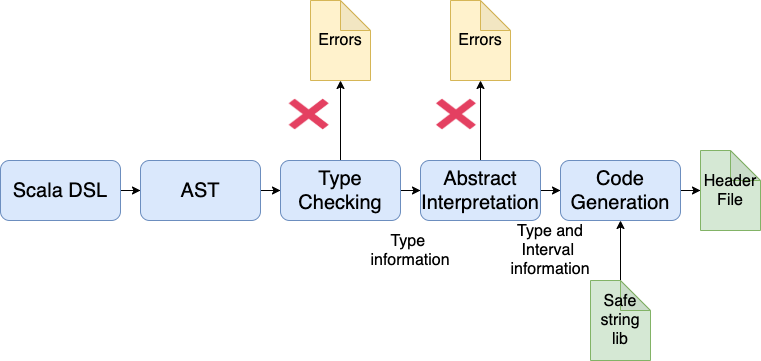
\includegraphics[width=\textwidth]{architecture.png}
  \caption{Diagram of the compiler pipeline}
  \label{fig:pipeline}
\end{figure}

\begin{figure}[h]
  \centering
  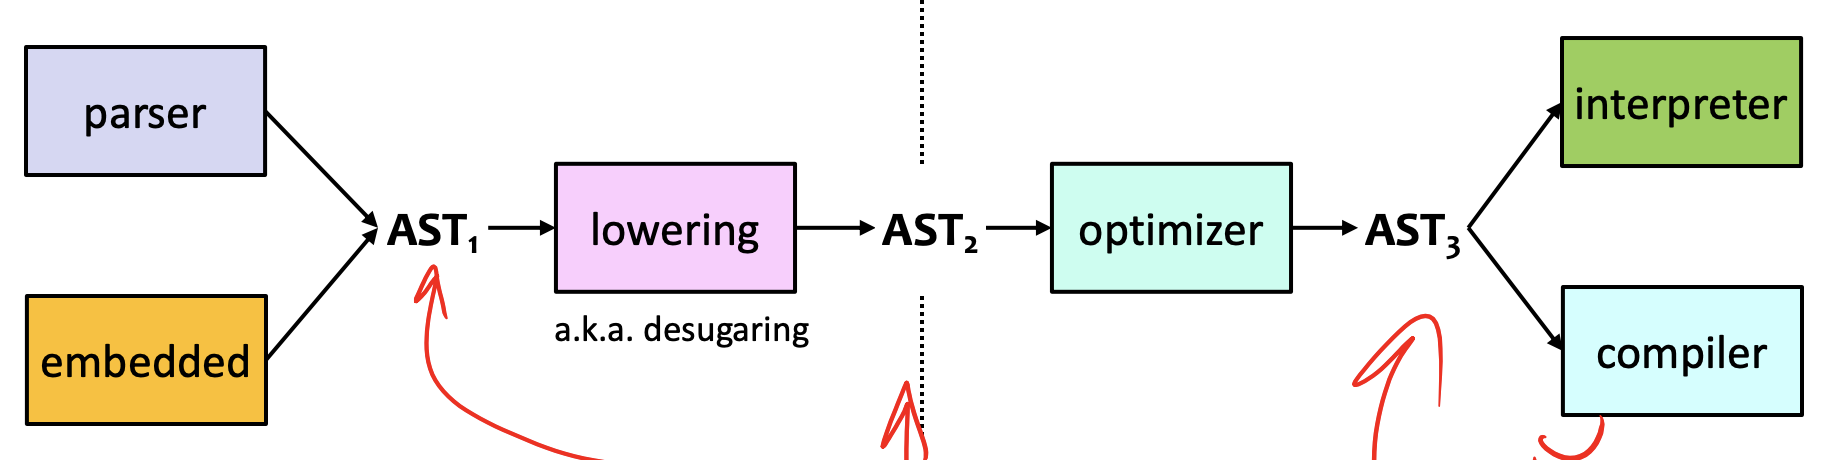
\includegraphics[width=\textwidth]{modern-compiler-pipeline.png}
  \caption{Diagram of the compiler pipeline. (Screenshot from the marked up lecture slides)}
  \label{fig:mdnpipeline}
\end{figure}


\subsection{Interface}

The interface of the compiler is shown as the \textit{Scala DSL} box in
figure \ref{fig:pipeline}. It is the equivalent of the \textit{embedded}
and \textit{parser} blocks of the pipeline shown in figure \ref{fig:mdnpipeline}.
Originally, I was using a lexer and parser to make the syntax similar to
C as shown in figures \ref{fig:forloopsyntax} and \ref{fig:functionsyntax}, but
I switched to a fluent-syntax style in scala. The two styles are shown with
equivalent code in figures \ref{fig:csyntax} and \ref{fig:fluentsyntax}.

\begin{figure}[h]
  \centering
  \begin{lstlisting}
num_iter scan_line (string clause_line)
  {
    for (lit : str_split (clause_line, " ") | num_iter literals )
    {
      ston(lit);
    }

    return literals;
  }
  \end{lstlisting}
  \caption{Original, C-familiar syntax using a lexer and parser}
  \label{fig:csyntax}
\end{figure}

\begin{figure}[h]
    \begin{lstlisting}
val scanner = 
      Function("scan_line")
        .returnType(IntIterT())
        .arg(Argument("clause_line").withType(StringT))
        .startFunction()
           .loop(
             ForEach("lit")
               .inExpr(Var("clause_line").split(" "))
               .withAcc(Variable("literals").withType(IntIterT()))
               .startFor()
                 .setAcc(Var("lit").ston)
               .endFor)
           .ret(Var("literals"))
        .endFunction
    \end{lstlisting}
  \caption{New, fluent-syntax interface in Scala}
    \label{fig:fluentsyntax}
\end{figure}

The fluent syntax is not fully defined for all language features.
I left the syntax as the last thing I worked on, so I only implemented
features from my easy and medium examples. Things like the if-statement
were not added to the syntax. The implementation of the syntax is
in the \href{https://github.com/Flandini/cse501project20au/blob/master/scala-dsl/dsl/src/main/scala/Syntax.scala}
{Syntax.scala file} in the repo. The example from figure \ref{fig:fluentsyntax} is at the bottom of that file.

\subsection{Typechecking}

The compiler does the usual typechecking (e.g., strings are not
being subtracted or multiplied). There are \href{https://github.com/Flandini/cse501project20au/blob/master/scala-dsl/dsl/src/main/scala/TypeCheck.scala#L29}{two passes} since multiple functions can be defined.
There are also some DSL specific checks like no recursive function
calls and the lower bound of a range is less than or equal to
the upper bound of the range. 

\subsection{Abstract interpretation}

The interval semantics and domain are defined in \href{https://github.com/Flandini/cse501project20au/blob/master/scala-dsl/dsl/src/main/scala/Interval.scala#L150}{this file}, and the analysis is implemented in \href{https://github.com/Flandini/cse501project20au/blob/master/scala-dsl/dsl/src/main/scala/SafetyChecks.scala}{this file}. 

I decided last-minute to switch to abstract interpretation
over symbolic execution. I felt that it would be easier to get
an abstract interpreter finished than it would be the symbolic
execution engine with all the tricky integer semantics. I also
think that for my DSL, the two are equally as precise. Also,
since all values are bounded and all programs terminate, widening
and narrowing are optimizations and not necessities which made
writing the abstract interpreter much easier; I just wrote an
interpreter using the interval domain and ride out loops.

I wrote most of the abstract interpreter last minute since I needed
to have at least the code generation working for the demo. The \href{https://github.com/Flandini/cse501project20au/blob/master/scala-dsl/dsl/src/main/scala/SafetyChecks.scala#L15}{code}
for this part of the project ended up \href{https://github.com/Flandini/cse501project20au/blob/master/scala-dsl/dsl/src/main/scala/SafetyChecks.scala#L218}{\textit{very} messy} as a result.
I also did not finish the semantics for any of the string and iterator
expressions not used in the sample programs. I also did not get
integer-promotion fully implemented in the abstract interpreter,
so the analysis is currently unsound.

The analysis is working pretty well though. Actually, well enough that it
caught problems in my sample programs that I hadn't caught. I originally planned to
demo both the \href{https://github.com/Flandini/cse501project20au/blob/master/samples/easy/single_line_dimacs_scanner.sal}{easy example}
and the \href{https://github.com/Flandini/cse501project20au/blob/master/samples/medium/array_average.sal}{medium example},
but the analyzer found issues with the medium example.

The analyzer found the potential div by zero when the numbers iterator
has length $0$. I changed the bound on the iterator to be $\{1, 50000\}$, but
then the analyzer complained about the potential truncation on the return
value since the analyzer says that \textit{averageish} is from the range
$[0, 12750000]$, but the return value is constrainted to $[0, 255]$. This
results from the interval analysis being too coarse; it does not associate
that the range of \textit{acc} is dependent on the range of the length of
the iterator \textit{numbers}--i.e., when numbers contains only 1 element
(and that element is constrained to $[0, 255]$), the analyzer still says
that the sum of all numbers could be $[0, 12750000]$.

\subsection{Code generation}

I also couldn't get all of code generation finished. I didn't get
if-statements and \href{https://github.com/Flandini/cse501project20au/blob/master/scala-dsl/dsl/src/main/scala/Codegen.scala#L242}{
some string and iterator expressions} finished. There is enough of it
finished though to get the easy and medium examples and some small
test cases generated. The code generation part was pretty easy though
since there are no optimizations, so given another 2-3 hours, I could
probably get it completely finished.

Most of the code generation just uses templates. For example, there is an
idiomatic way of safely splitting strings in C (\textit{str\_split} in the DSL),
so the DSL just spits out a \href{https://github.com/Flandini/cse501project20au/blob/master/scala-dsl/dsl/src/main/scala/Codegen.scala#L267}{string template for a \textit{str\_split} expression}.
Variable names might need to be changed, and RHS-value type expressions might need to be
stored, but the template is always the same.

Some code shouldn't be generated and stuck in a function body using the templating-method.
The code might be too long or too unreadable if inserted in place, so those go in the
\href{https://github.com/Flandini/cse501project20au/blob/master/scala-dsl/dsl/src/main/scala/lib.h#L7}{pre-defined
  safe string library} where they are static and inlined.


The generated code for figures \ref{fig:csyntax} and \ref{fig:fluentsyntax}
is given in figure \ref{fig:gencode}.

\begin{figure}[h]
  \centering
  \begin{lstlisting}
int32_t* scan_line(char* clause_line) {
  char* lit;
  char* delim0 = " ";
  char* pass_through_0 = clause_line;
  char* pass_through_0_dup_0 = strdup(pass_through_0);
  char** iterator0 = str_split(pass_through_0_dup_0, delim0);
  int32_t* literals  = calloc(char_iter_length(iterator0), sizeof(int32_t));

  for (uint32_t i_0 = 0; (lit = iterator0[i_0]); ++i_0) {
      literals[i_0] = atoi(lit);
  }

  free (pass_through_0_dup_0);
  return literals;
}
  \end{lstlisting}
  \caption{Code generated for the \href{https://github.com/Flandini/cse501project20au/blob/master/samples/easy/single_line_dimacs_scanner.sal}{easy sample program} shown in \ref{fig:csyntax} and
    \ref{fig:fluentsyntax}. Spacing was originally messed up, so I've prettified the
    indents.}
  \label{fig:gencode}
\end{figure}

The \textit{pass\_through\_0} variable is just an intermediate value; the DSL assigns RHS values
(expressions) to these indexed variables so that these expressions can later be referred
to. This needs to be done to some expressions to avoid re-computing them.

The code generator isn't smart enough to insert the \textit{free} call for \textit{iterator0} at
the end of the function, so \textbf{there is a memory leak}. There would have to be more
analysis to figure out what is safe to free relative to what is being returned, or all strings
would have to be copied on assignment.

\section{Discussion}
\label{sec:discussion}

\subsection{Things not finished}

All of the type checker and AST are finished. Abstract interpretation is very sloppy
and is not implemented for some string and iterator expressions, if-statements, and
integer promotion. Code generation is also not finished for the same string and iterator
expressions as well as if-statements. The hard goal of being able to declare multiple
functions in the DSL as a library is also not fully implemented. The type checker and AST
allow this, but the abstract interpreter and code gen can't handle this. 

\subsection{Neat features}

\begin{itemize}
  \item I am pretty proud of myself for \href{https://github.com/Flandini/cse501project20au/blob/master/scala-dsl/dsl/src/main/scala/Interval.scala#L2}{using TypeLevel's algebra library for its \textit{Lattice} trait} in defining the interval domain.

  \item I am pretty proud of the \href{https://github.com/Flandini/cse501project20au/blob/master/scala-dsl/dsl/src/main/scala/TypeCheck.scala#L99}{monadic style of the type checker}.

  \item I am not used to functional programming or typing (my first exposure to the lambda calculus and typed lambda calculus was this course), so I'm also pretty proud that I did it all in Scala.

  \item I am pretty proud of the \href{https://github.com/Flandini/cse501project20au/blob/master/scala-dsl/dsl/src/main/scala/SafetyChecks.scala#L480}{interval analysis of the \textit{ston} and \textit{ntos} (string-to-number and number-to-string) expressions}. I originally thought that this would be pretty difficult, but writing the code to bound based on potential number of digits or characters was fun.
\end{itemize}

\subsection{Mistakes}

I did not define the project well enough in the beginning, and my sample programs
were not (and still are not) concrete enough. I also made the project too big and
difficult given the course given the scope, time, and that this is also not a
research project.


\subsection{What I would do differently}
Two things: 1) I would find concrete examples of buggy, C-string code I wanted
to rewrite in the DSL, and 2) build the DSL/compiler starting much smaller.

I am pretty familiar with string and integer related C and C++ vulnerabilities,
and thinking that I am pretty familiar with these vulnerabilities made me
work backwards from the solution to the problem. I think I could've had a much
more concrete and better problem definition if I looked at some buggy, C-string
code, formed the problem and some examples, and then built my DSL as solution.
I think I could have saved myself 2-3 weeks worth of work.

I would also only handle string and integer expressions first. I would build
the AST, typechecker, absint, and code generation for these first, and then
slowly build out to statements, control flow, functions, and then multiple
functions. These were the most stressful and important parts. I think that
doing this would have been much more efficient than building all of the
type checker for all AST nodes and then all of the abs int for all AST nodes
and so on.

\subsection{What knowledge or skill would have helped with the project}

I would have liked a homework or a lecture over engineering a more difficult
interpreter. I did all of the Monads for Functional Programming and Essence
of Functional Programming examples, but they only touched on one monad at a time
and some simple semantics. I felt those papers/tutorials were helpful for learning
monads, but they didn't bridge the gap between using one monad and building a complex
or real interpreter that might combine monads or have really deeply nested for blocks.
I ended up learning about things like monad transformers and free monads later on, and
I think this might've helped, but I still don't understand them that well.

\end{document}
